\documentclass[tikz]{standalone}
\date{}
\usepackage{amsmath,amsthm,amssymb}
\usepackage{xcolor}
\usepackage{tikz}
\usepackage[siunitx]{circuitikz}
\usepackage{tikz-3dplot}
\usepackage{ifthen}
\tikzset{isometricXYZ/.style={x={(-0.866cm,-0.5cm)}, y={(0.866cm,-0.5cm)}, z={(0cm,1cm)}}}
\usetikzlibrary{arrows,decorations.pathmorphing,positioning,fit,trees,shapes,automata,calc,intersections,decorations.markings,patterns,graphs,quotes,plotmarks}
%\usepackage{algorithm}
%\usepackage{algorithmic}
\newcommand{\R}{\mathbb{R}}
\newcommand{\F}{\mathbb{F}}
\newcommand{\bmat}[1]{\begin{bmatrix}#1\end{bmatrix}}
\newcommand{\xth}[1]{{#1}^{\mathrm{th}}}
\newcommand{\pd}[2]{\frac{\partial #1}{\partial #2} }
\newcommand{\pdd}[2]{\frac{\partial^2 #1}{\partial #2^2}}
\newcommand{\myitemsep}{\setlength\itemsep{-0.25em}}
\newcommand{\bigpar}[1]{\left( #1\right)}
\tikzset{myedge/.style={ thick,->,>=stealth',inner sep=0pt,outer sep=3pt}}
\tikzset{hv path/.style= {to path={-| (\tikztotarget)}}}
\tikzset{vh path/.style= {to path={|- (\tikztotarget)}}}

%%%%%%%%%% Using shift and rotate around:

\newcommand{\spring}[4]{
\path[shift={#1},rotate={#2},fill = white,opacity=1.0] (-0.25,-0.5) rectangle (0.25,0.5); % cover
\draw[thick,shift={#1},rotate={#2}] (0,0.5) -- +(0.25,-0.1) -- +(-0.25,-0.2)-- +(0.25,-0.3)-- +(-0.25,-0.4)-- +(0.25,-0.5)-- +(-0.25,-0.6)-- +(0.25,-0.7)-- +(-0.25,-0.8)-- +(0.25,-0.9) -- +(0,-1.0);
\draw[thick,shift={#1},rotate={#2}] (#3,0) node {#4};
}
\newcommand{\ground}[3]{
\draw[thick,shift={#1},rotate={#2}] (-0.5*#3cm,0) -- (0.5*#3cm,0);
\path[thick,shift={#1},rotate={#2},pattern=north west lines] (-0.5*#3cm,0) rectangle (0.5*#3cm,0.2);
}
\newcommand{\dashpot}[4]{
\path[shift={#1},rotate={#1},fill = white,opacity=1.0] (-0.25,0) rectangle (0.25,0.15);
\path[shift={#1},rotate={#1},draw,thick] (0,0) -- +(0.25,0) -- +(0.25,0.25) +(0.15,0.15) -- +(-0.15,0.15)  +(-0.25,0.25) -- +(-0.25,0) -- +(0,0);
\draw[thick,shift={#1},rotate={#1}] (#3,0) node {#4};
}
\newcommand{\mydashpot}[5]{
\begin{scope}[xshift=#1cm,yshift=#2cm,rotate=#3]
	\path[fill = white,opacity=1.0] (-0.25,0) rectangle (0.25,0.15);
	\path[draw,thick] (0,0) -- +(0.25,0) -- +(0.25,0.25) +(0.15,0.15) -- +(-0.15,0.15)  +(-0.25,0.25) -- +(-0.25,0) -- +(0,0);
	\node at (#4,0) {#5};
	\end{scope}
}
\newcommand{\lapof}[1]{\mathcal L \left\{ #1 \right\}}
\newcommand{\lapinv}[1]{\mathcal L^{-1} \left\{ #1 \right\}}
\newcommand{\evalat}[2]{\left. #1 \right|_{#2}}
\newcommand{\myarr}[3]{(-#2:#1) arc (-#2:#2:#1) node[#3] }
\newcommand{\mc}[1]{\mathcal{#1}}
\newcommand{\mred}[1]{\textcolor{red}{[#1]}}
\newcommand{\myco}[2]{\bigpar{ \frac{#1}{#2} }}
\newcommand{\tc}[2]{{#1}{#2}}
\newcommand{\mcb}[1]{{\color{blue}#1}}
\newcommand{\mcr}[1]{{\color{red}#1}}
\newcommand{\mcg}[1]{{\color{green!70!black}#1}}
\usepackage{hyperref}
\hypersetup{colorlinks=true,
linkcolor=blue,          % color of internal links
        citecolor=green,        % color of links to bibliography
          filecolor=magenta,      % color of file links
           urlcolor=blue           % color of external links
}

%\tikzstyle{name}=[options]
\def\nodespx{6cm}\def\nodespy{1.7cm}
\tikzstyle{mynode}=[thick,rounded corners = 0.1cm,draw,minimum size=0.375cm,align=center]
\tikzstyle{myedge} = [thick,->,>=stealth',outer sep=0pt,inner sep=0pt]
\tikzstyle{nodraw}=[draw=none]
\tikzstyle{alignc}=[align=center]
\newcommand{\tw}{text width}
\newcommand{\mw}{minimum width}
\newcommand{\mh}{minimum height}
\begin{document}
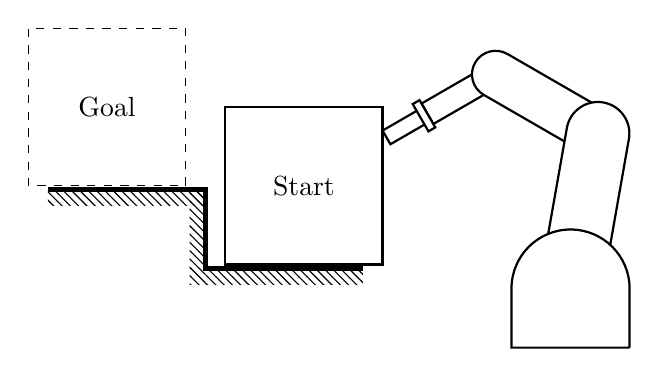
\begin{tikzpicture}[>=stealth']
\coordinate (j1) at (0,0);
\def\qa{80}\def\qb{150}\def\qc{210}
\def\la{2.0}\def\lb{1.5}\def\lc{1.0}
\coordinate (j2) at ($(j1)+(\qa:\la)$) ;
\coordinate (j3) at ($(j2)+(\qb:\lb)$) ;
\coordinate (ee) at ($(j3)+(\qc:\lc)$) ;
\coordinate (j4) at (4,0);
%%% Third moving link:
\draw[shift=(j3),rotate=\qc,fill=white,thick] (0,-0.15*\lc) rectangle (\lc,0.15*\lc);
\draw[shift=(ee),rotate=\qc-90,fill=white,thick] (-0.1,0) rectangle (0.1,0.6) coordinate (task);
\draw[shift=(j3),rotate=\qc,fill=white,thick] (\lc,-0.2*\lc) rectangle ++(0.1*\lc,0.4*\lc);
%% Second moving links
\draw[shift=(j2),rotate=\qb,fill=white,thick] (0,0) ++(90:0.2*\lb) -- ++(0:\lb) arc (90:-90:0.2*\lb) -- ++(-180:\lb);
%% first moving links
\draw[shift=(j1),rotate=\qa,fill=white,thick] (0,0) ++(90:0.2*\la) -- ++(0:\la) arc (90:-90:0.2*\la) -- ++(-180:\la);
%% base
\draw[fill=white,thick,xscale=0.75,yscale=0.75] (j1) +(1,-1) -- ++(-1,-1) -- ++(0,1) arc (180:0:1) -- ++(0,-1);
%%% Task:
\draw[thick] (task) ++(0,0.3) rectangle ++(-2,-2) coordinate (boxcorner) ++ (-0.25,-0.05) coordinate (stepcorner);
\draw[pattern=north west lines,draw=none, thick] (stepcorner) rectangle ++(2,-0.2);
\draw[pattern=north west lines,draw=none, thick] (stepcorner) rectangle ++(-0.2,-0.2);
\draw[pattern=north west lines,draw=none, thick] (stepcorner) rectangle ++(-0.2,1);
\draw[pattern=north west lines,draw=none, thick] (stepcorner)++(0,1) rectangle ++(-2.0,-0.2);
\draw[ultra thick] (stepcorner) ++(2,0) -- ++(-2,0) -- ++(0,1) -- ++(-2.0,0); 
\draw (boxcorner) ++(1,1) node {Start};
\draw[dashed] (boxcorner) ++(-0.5,1) rectangle ++(-2,2) ++(1,-1) node{Goal};		
\end{tikzpicture}
 \end{document}
 
 
% Rewards Node
%\draw (rewardloc) node(rew)[mynode,draw=none,text width=3cm,align =center]{Reward Model \\ (Section~\ref{sssec:rewardmodels})};
%%% green SOTA as a node
%\draw (cmgmploc) node(sotanode)[mynode,\mw=4cm,\mh = 6cm,fill = green!10,dashed]{};
%\draw (sotanode.north west) node[above right,green!70!black]{State-of-the-Art Planner};
